
\documentclass[varwidth,border=20pt]{standalone}
\usepackage{tikz}
\usetikzlibrary{arrows.meta}
\usetikzlibrary{shapes}
\usetikzlibrary{backgrounds,shadows}

\begin{document}  
%Process: SIMPLEPROCESS
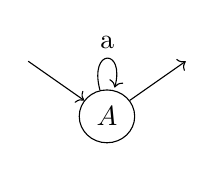
\begin{tikzpicture}[baseline, y=-0.7cm]

    % Declare the states
    \node[draw, ellipse] at (0, 0) (A0) {$A$};

    % Declare edges
    \draw[->] (A0) edge[loop above] node[midway, above] {a} (A0);

    % Declare initial edges
    \draw[->] (-1, -1) -- (A0) node[midway] {};

    % Declare final edges
    \draw[->] (A0) -- (1, -1) node[midway] {};

\end{tikzpicture}
\vspace{2em}
\end{document}